\documentclass[12pt]{report}

% Times New Roman font
\usepackage{mathptmx}
\usepackage[T1]{fontenc}
\usepackage{graphicx} % For images
\usepackage{geometry} % To adjust margins
\geometry{a4paper, margin=1in}
\usepackage{tikz}
\usepackage{graphicx}
\usepackage[margin=1in]{geometry}
\usepackage{titlesec}
\usepackage{lmodern} % For improved fonts
\usepackage{array}
\usepackage{ragged2e}
\usepackage{makecell}

\begin{document}

\begin{titlepage}
    \clearpage 
\pagestyle{empty}

% TikZ border box
\begin{tikzpicture}[remember picture,overlay,inner sep=0,outer sep=0]
   \draw[black!70!black,line width=5pt] 
   (-1.5,2) -- (-1.5,-24) -- (15.5,-24) -- (15.5,2) -- (-1.5,2);
   \draw[black!70!black,line width=0.2pt] 
   (-1.3,1.8) -- (-1.3,-23.8) -- (15.3,-23.8) -- (15.3,1.8) -- (-1.3,1.8);
\end{tikzpicture}

% Centered content
\begin{center}

% Title nicely centered
{\fontsize{16}{16}\selectfont \bf SUSTAINABLE EV CHARGING STATION COMBINING WIND TURBINE AND SOLAR PHOTOVOLTAIC TECHNOLOGIES}\\[0.4cm]

\hspace*{-0.9cm}{\large \textit{A Project Report submitted in partial fulfillment of the requirements for award of the degree}}\\[0.2in]

{\fontsize{16}{16}\selectfont \bf BACHELOR OF ENGINEERING}\\[0.2in]

{\large \bf \textit{In}} \\[0.2in]

{\fontsize{16}{16}\selectfont \bf ELECTRONICS \& TELECOMMUNICATION} \\[0.2in]

{\large \bf \textit{Of}} \\[0.1in]

{\fontsize{16}{16}\selectfont SAVITRIBAI PHULE PUNE UNIVERSITY}\\[0.3in]

% Student names and exam numbers in tabular for alignment
{\large \bf \textit{By}}\\[0.1in]

\begin{tabular}{>{\bfseries}l @{\hspace{2cm}} >{\bfseries}l}
Bhavesh Gaikwad & Exam No.  B400230454\\
Nilesh Khilari & Exam No. B400230519\\
Sanket Sonje & Exam No. B400230634\\
\end{tabular}

\vspace{0.5in}
{\Large \bf \textit{Under the Guidance of}}\\[0.2in]
{\Large \bf Prof. P. M. Dahale }\\[0.3in]

% College logo

\includegraphics[scale=0.7]{clg logo.jpg}\\[0.3in]

{\normalsize \bf Department of Electronics \& Telecommunication Engineering }\\[0.1in]
{\large \bf Sinhgad College of Engineering,}\\[0.05in]
{\large \bf Vadgaon (BK), Pune - 411041}\\[0.05in]
{\large \bf 2025-2026}

\end{center}


\end{titlepage}

\begin{Certificatepage}
\clearpage
\thispagestyle{empty}
\begin{center}
    
\includegraphics[scale=1]{clg logo.jpg}
    
    \vspace{0.3in}
    {\fontsize{22}{22}\selectfont \bf CERTIFICATE}
    
    \vspace{0.3in}
    {\fontsize{12}{12}\selectfont This is to certify that the project report entitled}
    
    \vspace{0.2in}
    {\fontsize{16}{16}\selectfont \bf "SUSTAINABLE EV CHARGING STATION
    COMBINING WIND TURBINE AND SOLAR PHOTOVOLTAIC TECHNOLOGIES"}
    
    \vspace{0.2in}
    {\large \bf \textit{Submitted }}
    \vspace{0.1in}
    {\large \bf \textit{by}}\\[0.3in]
   \begin{center}
\vspace{0.2in}
\begin{tabular}{c}
\textbf{Bhavesh Gaikwad \hspace{1.7cm} Exam No. B400230454}\\
\textbf{Nilesh Khilari  \hspace{2.5cm} Exam No. B400230519}\\
\textbf{Sanket Sonje    \hspace{2.7cm} Exam No. B400230634}\\
\end{tabular}
\end{center}


\vspace{2mm}
\noindent
\begin{justify}
Have successfully completed their Project under the supervision of \textbf{Prof. P. M. Dahale} for the partial fulfillment of Bachelor of Engineering \textbf{Electronics and Telecommunication} of Savitribai Phule Pune University. This work has not been submitted elsewhere for any degree.
\vspace{25mm} 

\noindent
\noindent
\begin{minipage}[t]{0.33\textwidth}
\centering
\textbf{Prof. P. M. Dahale}\\
Guide
\end{minipage}\hfill
\begin{minipage}[t]{0.33\textwidth}
\centering
\textbf{Prof. C. R. Kuwar}\\
Project Coordinator

\end{minipage}\hfill
\begin{minipage}[t]{0.33\textwidth}
\centering
\textbf{Dr. R. S. Kawitkar}\\
HOD E\&TC
\end{minipage}
 
\vspace{25mm} 

\noindent
\begin{minipage}[t]{0.33\textwidth}
\centering
External Examiner
\end{minipage}\hfill
\begin{minipage}[t]{0.33\textwidth}
\centering
\textbf{}\\

\end{minipage}\hfill
\begin{minipage}[t]{0.33\textwidth}
\centering
\textbf{Dr. S. D. Lokhande}\\
Principal SCOE
\end{minipage}

\tableofcontents
\newpage

\listoffigures
\addcontentsline{toc}{chapter}{List of Figure}
 
\newpage

\chapter*{Abstract}
\addcontentsline{toc}{chapter}{Abstract}

    
With the rapid growth of electric vehicles (EVs), the demand for clean, reliable, and sustainable charging infrastructure is increasing significantly. This project presents a Sustainable EV Charging Station Combining Wind Turbine and Solar Photovoltaic Technologies for efficient and eco-friendly electric vehicle charging. The system integrates two renewable energy sources—solar photovoltaic (PV) panels and wind turbines—to generate electricity and provide uninterrupted power for EV charging. \vspace{0.5cm} % Space between paragraphs (optional)

The proposed system consists of solar PV panels, a wind turbine, charge controllers, a battery storage unit, voltage and current monitoring sensors, and an EV charging module. The solar panels convert sunlight into electrical energy, while the wind turbine generates power from wind energy. The energy produced from both sources is regulated through charge controllers and stored in a battery bank for continuous availability. Monitoring sensors continuously track system performance, battery status, and power generation parameters.\vspace{0.5cm} % Space between paragraphs (optional)

This hybrid renewable energy-based charging station reduces dependence on conventional grid electricity and minimizes carbon emissions associated with transportation. The combination of solar and wind energy improves overall system reliability and energy availability compared to single-source renewable systems. The proposed solution is suitable for highways, smart cities, parking facilities, educational campuses, and remote locations where sustainable energy solutions are required.\vspace{0.5cm} % Space between paragraphs (optional)

The project offers an environmentally friendly, cost-effective, and scalable approach to EV charging infrastructure. By combining renewable energy generation, energy storage, and intelligent monitoring, the system contributes to the development of sustainable transportation and supports the global transition toward clean energy and green mobility.
 
\newpage


\chapter*{Acknowledgements}
\addcontentsline{toc}{chapter}{Acknowledgements}

\setlength{\parindent}{0pt} % Remove indentation for new paragraphs

We are feeling very humble in expressing my gratitude. It will be unfair to bind the precious help and support which we got from many people in few words. But words are the only media of expressing one’s feelings and my feeling of gratitude is absolutely beyond these words. It would be my pride to take this opportunity to say the thanks.  

\vspace{0.5cm} % Space between paragraphs (optional)

Firstly, we would thank our beloved guide \textbf{Prof. P. M. Dahale} for his valuable guidance, patience, and support; He was always there to force us a bit forward to get the work done properly and on time. He has always given us freedom to do project work and the chance to work under his supervision. 

\vspace{0.5cm} % Space between paragraphs (optional)

We would like to express our sincere thanks to \textbf{Prof. C. R. Kuwar}, project coordinator, Department of E\&TC, for his constant encouragement in the fulfillment of the project work. We would also like to express our sincere thanks to \textbf{Dr. R. S. Kawitkar}, \textbf{Head}, Department of E\&TC, for his cooperation and useful suggestions. We would also like to thank \textbf{Dr. S. D. Lokhande}, \textbf{Principal, Sinhgad College of Engineering}. He always remains a source of inspiration for us to work hard and dedicatedly.

\vspace{0.5cm} % Space between paragraphs (optional)

It is the love and blessings of our families and friends which drove us to complete this project work.

\vspace{0.5cm} % Space before "Thank you all!" to create a gap

Thank you all!

\vspace{2cm}
\begin{flushright}
\textbf{Bhavesh Gaikwad} \\
\textbf{Nilesh Khilari} \\
\textbf{Sanket Sonje}
\end{flushright}
\setlength{\parindent}{15pt} % Revert to default indentation (adjust value as necessary)





\newpage

\chapter*{Abbreviations}
\addcontentsline{toc}{chapter}{Abbreviations}

    \item \textbf{AC} – Alternating Current
    \item \textbf{DC} – Direct Current
    \item \textbf{ESP} – Embedded Serial Peripheral
    \item \textbf{ESP32} – Espressif Systems 32-bit Microcontroller
    \item \textbf{EV} – Electric Vehicle
    \item \textbf{GPIO} – General Purpose Input/Output
    \item \textbf{RFID} – Radio Frequency Identification
    \item \textbf{PV} – Photovoltaic
    \item \textbf{IoT} – Internet of Things
    \item \textbf{IR} – Infrared Sensor
    \item \textbf{LCD} – Liquid Crystal Display
    \item \textbf{SOC} – State of Charge
     
\newpage

\chapter{Introduction}


\section{Introduction}

\setlength{\parindent}{} % Remove indentation for new paragraphs

The Sustainable EV Charging Station Combining Wind Turbine and Solar Photovoltaic Technologies project aims to develop an environmentally friendly and reliable charging infrastructure for electric vehicles (EVs) using renewable energy sources. With the increasing adoption of electric vehicles worldwide, the demand for efficient and sustainable charging stations has grown significantly. Conventional charging stations primarily depend on grid electricity, which may be generated from fossil fuels and contribute to environmental pollution..

\vspace{10pt} % Space between paragraphs (optional)

This project proposes a hybrid renewable energy-based charging station that combines solar photovoltaic (PV) panels and wind turbines to generate clean electrical energy. The integration of these two renewable energy sources ensures continuous power generation, as solar energy is available during daytime while wind energy can be harnessed whenever sufficient wind is present. The generated energy is regulated through charge controllers and stored in a battery bank for future use.

\vspace{10pt} % Space between paragraphs (optional)

The system utilizes solar PV panels to convert sunlight into electrical energy and wind turbines to convert wind energy into electricity. A battery storage system is incorporated to store excess energy and provide uninterrupted power supply for EV charging. Monitoring sensors are used to measure parameters such as voltage, current, battery status, and energy generation. An LCD display can be used to display real-time system information and charging status

\vspace{10pt} % Space between paragraphs (optional)

The primary objective of the project is to develop a sustainable charging solution that reduces dependence on conventional power sources and promotes the use of renewable energy. The hybrid energy system improves reliability and efficiency compared to single-source renewable charging stations. Additionally, the system can be deployed in remote areas, highways, parking facilities, educational campuses, and smart cities where access to grid electricity may be limited.

 


\setlength{\parindent}{15pt} % Revert to default indentation (adjust value as necessary)

\newpage
\section{Aim}


The aim of the \textbf{Sustainable EV Charging Station Combining Wind Turbine and Solar Photovoltaic Technologies} project is to design and develop an efficient, environmentally friendly, and reliable electric vehicle charging system powered by renewable energy sources. The project focuses on integrating solar photovoltaic (PV) panels and wind turbines to generate clean electrical energy for EV charging while reducing dependence on conventional grid power.

\vspace{10pt} % Space between paragraphs (optional)

\section{Objectives}
The objective of the Sustainable EV Charging Station Combining Wind Turbine and Solar Photovoltaic Technologies project is to develop a hybrid renewable energy-based EV charging station that ensures reliable power generation and efficient energy utilization. The system combines solar and wind energy sources to support sustainable transportation and reduce reliance on fossil-fuel-based electricity.

\vspace{10pt} % Space between paragraphs (optional)

\textbf{Some of the main goals of the project are}

\vspace{10pt} % Space between paragraphs (optional)
1. \textbf{Renewable Energy Generation:} The system utilizes solar photovoltaic panels and wind turbines to generate clean and sustainable electrical energy. The objective is to maximize the use of renewable resources and reduce greenhouse gas emissions.

\vspace{10pt} % Space between paragraphs (optional)
2. \textbf{Continuous EV Charging Supply:} The hybrid energy system ensures a reliable and uninterrupted power supply for electric vehicle charging by combining solar and wind energy sources, which complement each other under varying weather conditions.

\vspace{10pt} % Space between paragraphs (optional)
3. \textbf{Energy Storage and Management:} A battery storage system is incorporated to store excess energy generated from renewable sources. The objective is to maintain energy availability during periods of low sunlight or insufficient wind speed and improve overall system efficiency.

\vspace{10pt} % Space between paragraphs (optional)
4. \textbf{Reduction of Grid Dependency:} The project aims to minimize dependence on conventional grid electricity by utilizing renewable energy sources, thereby reducing operating costs and promoting energy independence.

\vspace{10pt} % Space between paragraphs (optional)
5. \textbf{Deployment in Remote Areas:} The charging station is designed to operate in locations where grid access may be limited or unavailable, making it suitable for highways, rural regions, parking facilities, educational campuses, and smart city applications

\newpage

\section{Block Diagram} % This is now properly numbered 1.4
\setlength{\parindent}{0pt} % Remove indentation for new paragraphs
\textbf{Input Elements:}

\vspace{10pt}
• \textbf{Solar Panel:} Converts sunlight into electrical energy. It acts as the primary renewable energy source for the charging station.

\vspace{10pt}
• \textbf{Windmill Generator:} Generates electrical energy from wind. It provides additional power when solar energy is insufficient.

\vspace{10pt}
• \textbf{Charge Controller:} Regulates the power received from solar panels and wind turbines. It protects the battery from overcharging and improves charging efficiency.

\vspace{10pt}
• \textbf{Battery:} Stores excess energy generated by renewable sources. It supplies backup power during low generation periods.

\vspace{10pt}
• \textbf{ESP32 Microcontroller:} Acts as the central controller of the system. It monitors charging operations and controls communication between different modules.

\vspace{10pt}
• \textbf{RFID Moduler:} Provides user authentication before charging starts. It ensures that only authorized users can access the charging station.

\vspace{10pt}
\textbf{Output Components:}

\vspace{10pt}
• \textbf{AC Charging:} Provides normal AC charging for electric vehicles. It is suitable for regular charging requirements.

\vspace{10pt}
• \textbf{DC Fast Charging:} Supplies high-power DC charging to EVs. It significantly reduces charging time.

\vspace{10pt}
• \textbf{Wireless Charging:} Charges vehicles without physical cables using electromagnetic induction. It offers convenience and ease of use.

\vspace{10pt}
• \textbf{Grid Power AC Charging:} Uses grid electricity for charging when renewable energy is insufficient. It ensures continuous charging service

\vspace{10pt}
\begin{figure}[h!]
    \centering
    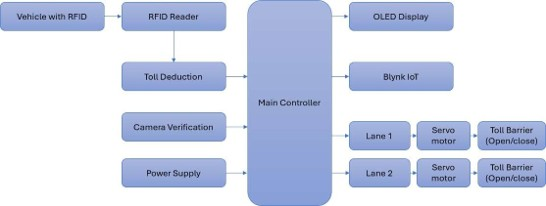
\includegraphics[width=0.6\textwidth]{block diagram.jpg} % Adjust the width to make the image smaller
    \caption{Block Diagram of Hybrid Solar–Wind Based EV Charging Station }
\end{figure}
\chapter{Literature Review}
\section{Introduction}
Electric vehicles (EVs) are becoming increasingly popular due to their environmental benefits and reduced dependence on fossil fuels. As the number of EVs grows, the demand for efficient, reliable, and sustainable charging infrastructure has also increased. Researchers have focused on integrating renewable energy sources such as solar and wind power with EV charging stations to reduce grid dependency and carbon emissions..

\vspace{10pt}
Earlier EV charging systems primarily relied on conventional grid electricity. Although these systems provided reliable charging, they increased the load on power grids and contributed indirectly to greenhouse gas emissions. To overcome these limitations, solar photovoltaic (PV) systems were introduced as renewable energy sources for EV charging. Solar-powered charging stations offered clean energy generation but faced challenges due to variations in sunlight availability.

\vspace{10pt}
To improve energy reliability, researchers proposed hybrid renewable energy systems combining solar and wind power. Wind turbines can generate electricity during periods of low solar radiation, thereby increasing overall energy availability. Several studies have shown that hybrid solar-wind charging stations provide better energy utilization, improved reliability, and reduced dependence on conventional energy sources.

\vspace{10pt}
Recent developments have incorporated battery energy storage systems to store excess renewable energy for later use. Battery storage helps maintain uninterrupted charging during unfavorable weather conditions and enhances system stability. Researchers have also explored energy management strategies to optimize power flow between renewable sources, battery storage, and the electrical grid.

\vspace{10pt}
The proposed project addresses these challenges by developing a Sustainable EV Charging Station that integrates solar photovoltaic technology, wind turbine generation, battery storage, RFID authentication, and ESP32-based intelligent control. The system aims to provide reliable, eco-friendly, and efficient charging for electric vehicles while reducing dependence on conventional grid power

\vspace{10pt}
\section{Literature Review}
\label{litrew}
\textbf{"Recent Advances in Smart Grid Architecture and Grid-Electric Vehicle-Charging Station Interaction" by Dongning Zhang.} This paper reviews smart grid technologies that are useful for optimal EV charging and for keeping energy distribution stable. Smart grids with features like smart metering and demand response alleviate grid stress and foster EV infrastructure. The study points out the contributions of EVs to the reduction of emissions and increasing the use of renewable energy. Case studies demonstrate that smart grid technologies improve EV charging efficiency, lower energy waste, and promote sustainable transportation. The paper 
forecasts that future developments will focus on advanced grid-EV integration, such as vehicle-to-grid (V2G) systems, to enhance 
grid stability and energy efficiency. 

\vspace{10pt}
\textbf{"Overview of Electric Vehicles Charging Stations in Smart Grids" by M. Wadi, W. Elmasry, M. Jouda, H. Shahinzadeh, and G. B. 
Gharehpetian.} This paper presents an incoherent insight into the technological make of EV charging stations within the smart grid, 
with emphasis on their inevitable role in facilitating the transition towards sustainable transportation. The paper deals with all the 
charging technologies such as Level 1, Level 2, DC Fast Charging, and wireless charging while addressing issues concerning the 
scalability of infrastructure, its integration with the grid, and interoperability. Then, the paper investigates how optimal placements 
for on-grid and off-grid charging stations can be found using a DC-DC converter, which would enhance charging efficiency. Finally, 
future trends for charging infrastructure are analyzed in the paper. 

\vspace{10pt}
\textbf{"Smart Environment: The Base for Energy Management Strategy-Based Scenario of a Solar Charging Station for Electric Vehicles" 
by Morteza Azimi Nasab, Mohammad Zand, P. Sanjeevikumar, Atif Iqbal and Baseem Khan.} The presented article concerns a solar 
charging station for EVs with Smart Energy Management in order to optimize costs and to be efficient. This paper shows how 
predictive analytics combined with automatic management strategies could be optimized using deep learning for forecasting the 
level of EV charging and Social Network Analysis used for EV behavior assessment. Tested on the IEEE 33-bus network, this 
proposed system will decrease energy consumption and emit a useful model for urban smart environments.

\vspace{10pt}
\textbf{“A Comprehensive Analysis: Integrating Renewable Energy Sources with Wire/Wireless EV Charging System for Green Mobility” 
by ,Ahmed Shahin, Almoataz Y. Abdelaziz, Azeddine Houari, Babak Nahid-Mobarakeh, Serge Pierrfederici, Fujin Deng, Sayed 
Abulanwar.} Integrating renewable energy sources with existing power grids can help manage the increased demand from EV 
charging, even if most charging occurs during off-peak hours. This paper reviews various EV charging methods, emphasizing grid
based charging with renewables. The most practical approach is large-scale renewable energy stations connected to the grid. The 
study also highlights challenges, particularly for wireless charging systems, like energy loss, coil alignment, and safe, efficient 
power transfer. It explores different wireless charger setups, especially a series-series configuration with photovoltaic integration, 
achieving around 98% efficiency and reliable operation despite grid fluctuations. 

\vspace{50pt}
\textbf{“Renewable Energy Power Assimilation to the Smart Grid and Electric Vehicles via Wireless Power Transfer Technology” by 
Hamid Allamehzadeh, Sarbagya Shakya.}This paper explores advancements in smart grid technologies and their role in integrating 
renewable energy sources, particularly wind and solar, for efficient electric power transfer. Wireless Power Transfer (WPT), 
especially Inductive Power Transfer (IPT), has emerged as a promising solution for charging electric vehicles (EVs) without physical 
connections, enhancing energy efficiency through magnetic resonance. As EV adoption grows, smart grid-connected and standalone 
wireless charging stations powered by renewables could support widespread EV usage and sustainable transportation. This review 
examines the opportunities and challenges of WPT in EV charging infrastructure, highlighting the potential for smart grids to 
revolutionize clean energy-driven mobility. 

\vspace{10pt}
\textbf{"Dynamic Wireless Charging for Inductive Power Transfer Systems in Electric Vehicles" by Ponmani Raja M., Karthik Chandran, 
and Jeyakannan.} The authors have studied DWC for EVs, which is the idea of charging vehicles while in motion. This technique 
tries to eliminate the shortcomings of conventional charging, such as longer recharging times and shorter driving distances. The 
principle of the proposed system is the installation of many inductive pads under roadways, enabling power transfer as moving 
vehicles drive on top.

\vspace{10pt}
\textbf{"Solar-Based Wireless Charging System for Electric Vehicles" by Aravind Kumar, Yashaswini N., and Rudresh S. J.} This paper 
discusses the integration of solar energy and wireless power transfer (WPT) for EV charging. Wireless charging through inductive 
coupling, an efficient and contactless energy transfer, is a promising aspect. Citing studies by Choi et al. (2014) and Rakhman et al. 
(2013), this paper illustrates the viability of these systems, while Uthaya Banu et al. (2018) highlight the environmental benefits of 
combining solar energy with WPT. Challenges like extended charging times and infrastructure limitations are discussed, alongside 
dynamic charging solutions as proposed by Magudeswaran et al. (2019). The paper suggests further research into the standardization 
of wireless charging of EVs, and its integration with smart grids, towards expanded infrastructure.

\vspace{10pt}
\textbf{Konstantina Dimitriadou, Nick Rigogiannis, Symeon Fountoukidis, Faidra Kotarela, Anastasios Kyritsis, and Nick Papanikolaou 
have authored "Current Trends in Electric Vehicle Charging Infrastructure; Opportunities and Challenges in Wireless Charging 
Integration".} This paper reviews EV charging infrastructure, examining conductive and wireless (inductive) charging advancements. 
This paper discusses wireless charging standards such as magnetic couplers and compensation networks and emerging power system 
architectures, including the Internet of Energy (IoE). Innovations such as dynamic and quasi-dynamic charging are analyzed, 
pointing out the role of smart control and communication in improving EV charging solutions. 

\vspace{40pt}
\\
\subsection{Method }
\label{met1}
A solar-powered EV charging system was proposed in one study that utilized photovoltaic panels and battery storage for charging electric vehicles. The system reduced dependence on conventional grid electricity but faced challenges during cloudy weather and nighttime due to limited solar energy generation.

\vspace{10pt}
Another project implemented a wind-powered EV charging station using small-scale wind turbines and energy storage units. The system generated clean energy effectively in windy regions but suffered from inconsistent power generation in areas with low wind speeds.

\vspace{10pt}
Researchers also developed hybrid renewable energy charging stations that combined solar and wind power sources. These systems improved energy availability and reliability by utilizing multiple renewable sources, reducing the limitations associated with individual energy generation methods.

\vspace{10pt}
Several studies incorporated battery energy storage systems to store excess renewable energy generated during peak production periods. The stored energy was later used for EV charging during periods of low renewable energy availability, improving system efficiency and reliability.

\vspace{10pt}
RFID-based authentication systems have been widely used in EV charging stations to provide secure access and user identification. These systems ensure that only authorized users can utilize charging facilities while maintaining charging records and usage information.

\vspace{10pt}
Recent research has focused on wireless EV charging technology using inductive power transfer. These systems eliminate the need for physical charging cables and improve user convenience, although challenges such as power transfer efficiency and system cost still remain.

\vspace{10pt}
Smart controllers such as ESP32 and IoT-based monitoring platforms have also been integrated into EV charging systems. These controllers enable real-time monitoring of battery status, charging parameters, and renewable energy generation while supporting remote management capabilities.

\vspace{10pt}
Current research trends emphasize the development of intelligent hybrid EV charging stations that integrate solar energy, wind energy, battery storage, wireless charging, and smart energy management systems. However, many existing solutions are expensive or depend heavily on grid infrastructure, highlighting the need for a cost-effective and sustainable charging station design.

\vspace{70pt}

\section{Summary}
A comprehensive review of existing research shows that EV charging stations have evolved through the integration of renewable energy sources such as solar photovoltaic systems, wind turbines, battery energy storage systems, and intelligent control technologies. These technologies have significantly improved the sustainability and efficiency of EV charging infrastructure while reducing dependence on conventional grid power.

\vspace{10pt}
Solar-powered charging stations provide clean and environmentally friendly energy but are affected by variations in sunlight availability. Similarly, wind-powered charging systems generate renewable energy effectively in suitable locations but depend heavily on wind conditions. To overcome these limitations, many researchers have proposed hybrid solar-wind systems that combine both energy sources to improve reliability and ensure continuous power generation.

\vspace{10pt}
Battery energy storage systems have been widely adopted to store excess renewable energy and provide backup power during periods of low energy generation. Smart energy management techniques further optimize the utilization of renewable resources and improve charging efficiency. RFID-based authentication systems and IoT-enabled controllers such as ESP32 have also enhanced user security, monitoring, and automation in modern charging stations.

\vspace{10pt}
Wireless charging technologies have recently gained attention due to their convenience and ease of use. However, challenges related to charging efficiency, infrastructure cost, and power transfer losses still exist. Many current solutions also require complex installations or substantial grid support, which increases implementation costs.

\vspace{10pt}
Overall, the literature indicates a growing trend toward sustainable, intelligent, and renewable energy-based EV charging infrastructure. The proposed project addresses these requirements by integrating solar photovoltaic panels, wind turbine generation, battery storage, RFID authentication, and ESP32-based intelligent control into a single system. This integrated approach aims to provide a reliable, cost-effective, secure, and environmentally friendly EV charging solution suitable for both urban and remote locations.

 
\\
\\
\chapter{Methodology}
\label{chapter3}

\section{Introduction}



To support the growing demand for clean and sustainable transportation, an EV charging system powered by renewable energy sources needs to be developed. This project follows a systematic approach that combines solar photovoltaic technology, wind energy generation, battery storage, ESP32-based control, and EV charging infrastructure to create an efficient and environmentally friendly charging station.
\vspace{10pt}
\par
The system utilizes solar panels and a windmill generator as primary energy sources. The electricity generated from these renewable sources is regulated through a charge controller and stored in a battery bank for continuous availability. An ESP32 microcontroller acts as the central controller, monitoring system operation, managing energy flow, and controlling charging activities.

\vspace{10pt}
The charging station incorporates an RFID module for user authentication and security. Once an authorized user is verified, the ESP32 activates the relay and enables the charging process. The system supports multiple charging methods, including AC charging, DC fast charging, and wireless charging. A grid connection is also provided as a backup source to ensure uninterrupted charging when renewable energy generation is insufficient.

\vspace{10pt}
This methodology emphasizes efficient energy management, reliable charging operation, and sustainable power utilization. The combination of renewable energy sources, battery storage, intelligent control, and secure access creates a practical solution for modern EV charging requirements. The following sections describe the system design, component integration, programming logic, and testing procedures used for successful implementation of the project.

 

\newpage
\section{Methodology 1}
\label{m1}

\subsubsection{Step-by-Step Development of the Sustainable EV Charging Station}
\vspace{10pt}

\subsubsection{\textbf{Step 1: System Planning and Objective Definition}}

The first step was to define the main objective of developing a sustainable EV charging station powered by solar and wind energy. A hybrid renewable energy approach was adopted to ensure continuous and eco-friendly charging of electric vehicles.

\subsubsection{\textbf{Step 2: Selection of Hardware Components}}

Hardware components were selected based on efficiency, reliability, and compatibility. The system uses solar panels, a windmill generator, charge controller, battery, inverter, ESP32 microcontroller, RFID module, relay, and EV charging unit.

\subsubsection{\textbf{Step 3: Circuit Integration and Connections}}

All components were connected according to the system design. The solar panel and windmill generator were connected to the charge controller and battery storage system, while the ESP32 was interfaced with the RFID module, relay, and charging unit.

\subsubsection{\textbf{Step 4: Programming and Logic Development}}

The ESP32 microcontroller was programmed using Arduino IDE to monitor and control charging operations. The program manages user authentication, charging control, battery monitoring, and energy management functions.

\subsubsection{\textbf{Step 5: Charging and Authentication System Setup}}

The RFID module was configured to authenticate authorized users before allowing access to the charging station. After successful verification, the ESP32 activates the relay and enables AC, DC fast, or wireless charging for the electric vehicle.

\subsubsection{\textbf{Step 6: Testing, Calibration, and Optimization}}

The complete system was tested under different operating conditions to evaluate charging performance, renewable energy generation, and battery operation. System parameters were optimized to improve charging efficiency, energy utilization, and overall reliability.

 

 
\vspace{10pt}
\par

\newpage

\subsection{Algorithms}
\label{algo}
The algorithm designed in this project aims to efficiently manage renewable energy generation and provide reliable charging for electric vehicles. The ESP32 microcontroller acts as the central controller, continuously monitoring energy generation, battery status, user authentication, and charging operations. The algorithm is designed to ensure efficient energy utilization, secure access, and uninterrupted charging service.

\vspace{10pt}
\par
Algorithm Steps:
\vspace{10pt}
\par
\textbf{Start the System:}

\par
Power is generated from the solar panel and windmill generator.The charge controller regulates the generated energy and stores it in the battery..
\vspace{10pt}
\par

\textbf{Initialize Components:}
\par
ESP32 initializes communication with the RFID module, relay, battery monitoring circuit, charging unit, and display system. All input/output pins and monitoring modules are configured..
\vspace{10pt}
\par

\textbf{Read Power Inputs:}
\par
Measure voltage and current from the solar panel and windmill generator.
Monitor battery voltage and charging status using ESP32 ADC pins.
\vspace{10pt}
\par

\textbf{Check Battery Status:}
\par
If battery voltage is above the predefined threshold, the system is ready for EV charging. If battery voltage falls below the minimum limit, charging is disabled and a low-battery warning is displayed.
\vspace{10pt}
\par

\textbf{Vehicle Detection and User Access:}
\par
The system continuously waits for a user request. The user scans an RFID card to access the charging station.
\vspace{10pt}
\par

\textbf{RFID Authentication:}
\par
Read RFID card information using the RFID module. If the card is valid, authorize the charging process. If the card is invalid, deny access and display "Unauthorized User".
\vspace{10pt}
\par

\textbf{Activate Charging System:}
\par
ESP32 activates the relay connected to the charging unit. Start EV charging through AC Charging, DC Fast Charging, or Wireless Charging mode.
\vspace{10pt}
\par

\textbf{Power Source Management:}
\par
Use renewable energy and battery storage as the primary power source. If renewable energy and battery power are insufficient, automatically switch to grid backup power..
\vspace{10pt}
\par

\textbf{Stop Charging:}
\par
When the charging process is completed or the user stops charging, ESP32 deactivates the relay
\vspace{10pt}
\par

\textbf{End of Process:}
\par
The system returns to idle mode and waits for the next user authentication and charging request.
\vspace{10pt}
\par



\newpage
\subsection{Flow Charts}
\label{fc}


\vspace{10pt} % Space between figure and text

\setlength{\parindent}{0pt} % Remove indentation for new paragraphs
\setlength{\parskip}{10pt} % Space between paragraphs

\noindent The flowchart describes the working process of the Sustainable EV Charging Station using Solar and Wind Power. The process starts with the initialization of the ESP32 microcontroller, which configures all connected modules including the RFID reader, battery monitoring circuit, relay, charging unit, and renewable energy sources.

The system continuously monitors power generated from the solar panel and windmill generator while checking the battery charging status. If sufficient energy is available, the charging station remains ready for operation. The user is then required to authenticate using an RFID card before accessing the charging facility.

By integrating solar energy, wind energy, battery storage, RFID authentication, and intelligent control through ESP32, the system provides a sustainable, secure, and reliable EV charging solution suitable for smart cities, highways, and remote locations


\begin{figure}[h!]
    \centering
    \includegraphics[width=0.6\textwidth]{flowchart BE pro.jpg} % Adjust the width to make the image smaller
    \caption{Flowchart of Hybrid Solar–Wind Based EV Charging Station}
\end{figure}

\newpage
\section{Methodology 2}
\label{m2}
During the initial stages of this project, an IoT-based smart monitoring system was considered for managing and monitoring the EV charging station remotely. Cloud platforms such as Firebase, AWS IoT, and Blynk were evaluated for storing charging data, monitoring battery status, tracking renewable energy generation, and providing remote access through mobile applications. The objective was to allow users and operators to monitor charging activities, energy consumption, and system performance from any location.

\par
This approach offered several advantages, including real-time monitoring, data logging, remote control, and energy usage analysis. Cloud-based platforms could also provide graphical visualization of solar power generation, wind energy production, battery status, and charging history. Such features would help improve energy management and user convenience.

\par
However, several challenges were identified during the evaluation process. Continuous internet connectivity is required for cloud communication, which may not always be available in remote or rural locations where EV charging stations are often needed. Dependence on internet services could affect system reliability and increase operational complexity.

\par
Another concern was the additional hardware and operational costs associated with cloud integration. The use of Wi-Fi routers, communication modules, and cloud subscription services would increase the overall project cost. Furthermore, transmitting charging and user data over the internet introduces cybersecurity and privacy concerns that require additional security measures.

\par
Considering these limitations, the project adopted a standalone ESP32-based control system. The ESP32 performs all monitoring, authentication, and charging control operations locally without depending on cloud services. This approach reduces power consumption, minimizes cost, improves reliability, and ensures uninterrupted operation even in locations with limited internet connectivity. As a result, the system provides a practical, sustainable, and efficient solution for EV charging using solar and wind energy.

\newpage

\chapter{Results \& Discussions}
\label{chapter4}

\section{Results}
\label{res}
\vspace{10pt}
\par
The Sustainable EV Charging Station prototype was successfully designed, implemented, and tested under controlled operating conditions. The system integrates renewable energy sources, battery storage, RFID-based authentication, and multiple charging technologies to provide a reliable and eco-friendly EV charging solution. The following results were obtained during testing and operation.
\vspace{10pt}
\par
\textbf{1. Renewable Energy Generation}
\par
The solar photovoltaic panel and wind turbine successfully generated electrical energy from sunlight and wind, respectively. The generated power was continuously monitored and regulated through the charge controller before being supplied to the battery storage system. During daytime operation, the solar panel contributed the majority of the energy, while the wind turbine generated supplementary power whenever sufficient wind was available. The hybrid energy generation approach improved overall system reliability by reducing dependence on a single renewable source. The results confirmed that combining solar and wind energy can provide a stable and sustainable power supply for EV charging applications.
\vspace{10pt}
\par
\begin{figure}[h!]
    \begin{center}
    %\centering
    \includegraphics[width=0.7\textwidth]{Renewable Energy.jpg} % Adjust the width to make the image smaller
    \caption{Renewable Energy Generation}
    \end{center}
    \vspace{10pt}
    \par
\textbf{ 2. Battery Charging and Energy Storage}
  \par
The battery storage system effectively stored excess energy produced by the solar panel and wind turbine. When renewable energy generation exceeded the charging demand, the surplus power was safely stored in the battery. During periods of low solar radiation, weak wind conditions, or nighttime operation, the stored energy was utilized to continue EV charging without interruption. The charge controller successfully protected the battery from overcharging and deep discharge conditions. Testing demonstrated that the battery storage unit plays a vital role in maintaining system stability and ensuring continuous availability of charging power.
\end{figure}

\par

\begin{figure}[h!]
    \begin{center}
     %\centering
    \includegraphics[width=1.0\textwidth]{Energy storage.jpg} % Adjust the width to make the image smaller
    \caption{Table of Battery Charging and Energy Storage}
    \end{center}
    \vspace{10pt}
    
    \par
   \textbf{3. RFID Authentication}
   \vspace{10pt}
   \par
The RFID authentication module successfully identified authorized users and restricted access to unauthorized individuals. When a valid RFID card was presented, the ESP32 verified the stored credentials and granted permission to start the charging process. Invalid or unregistered RFID cards were immediately rejected, and the charging system remained disabled. This feature enhanced the security of the charging station and prevented unauthorized energy usage. The authentication process was fast, reliable, and user-friendly, making it suitable for public and private charging stations.
\end{figure}
\vspace{10pt}
\par

\begin{figure}[h!]
    \begin{center}  
    %\centering
    \includegraphics[width=0.7\textwidth]{EV RFID1.jpg} % Adjust the width to make the image smaller
    \caption{RFID Authentication}
    \end{center}
    \vspace{10pt}
    \par
   \textbf{4. EV Charging Operation}
    \vspace{10pt}
    \par
The EV charging system functioned successfully after user authentication. The ESP32 activated the relay and supplied power to the charging unit. Different charging modes, including AC Charging, DC Fast Charging, and Wireless Charging, were tested and operated effectively. The charging process was continuously monitored to ensure safe operation and efficient energy utilization. Charging status information was displayed to the user, providing real-time feedback regarding charging activity. The results confirmed that the system can support multiple charging methods while maintaining reliable performance.
\end{figure}
\begin{figure}[h!]
    \begin{center}  
    %\centering
    \includegraphics[width=0.7\textwidth]{EV wind1.jpg} % Adjust the width to make the image smaller
    \caption{EV Charging Operation}
    \end{center}
    \vspace{10pt}
    \par
  \textbf{  5. Grid Backup Operation}
   \vspace{10pt}
    \par
The grid backup feature was successfully tested under conditions of insufficient renewable energy generation. Whenever solar and wind power, along with battery storage, could not satisfy the charging demand, the system automatically switched to grid power through the Main MCB. This transition occurred smoothly without interrupting the charging process. The automatic backup mechanism ensured continuous charging service even during unfavorable weather conditions. The test results demonstrated that integrating grid backup significantly improves the reliability and practicality of the charging station.
\end{figure}
\begin{figure}[h!]
    \begin{center}  
    %\centering
    \includegraphics[width=0.7\textwidth]{EV GRID1.jpg} % Adjust the width to make the image smaller
    \caption{Grid Backup Operation}
    \end{center}
    \vspace{10pt}
    \par
  \textbf{ }
   \vspace{10pt}
    \par

\vspace{10pt}
\par
\end{figure}
\clearpage

\section{Discussions}
\label{dis}
\vspace{10pt}
\par
The results demonstrate that the proposed Sustainable EV Charging Station effectively combines solar and wind energy to provide reliable and eco-friendly charging for electric vehicles. The integration of renewable energy sources, battery storage, RFID security, and ESP32-based control improved system efficiency and reduced dependence on conventional grid electricity.

\vspace{10pt} 
\par
However, some challenges and potential areas of improvement were noted:

\vspace{10pt}
\par 
\textbf{Renewable Energy Variability:} Power generation depends on sunlight intensity and wind speed. During unfavorable weather conditions, renewable energy production decreases.

\vspace{10pt} 
\par 
\textbf{Battery Capacity Limitation}\textbf{:} The charging duration depends on the available battery capacity. Larger battery banks can improve backup performance and charging availability.

\vspace{10pt}
\par
\textbf{Charging Time:} Although DC fast charging reduces charging time, AC charging requires a longer duration for full battery charging.

\vspace{10pt} \\
\par
\textbf{System Cost:} The initial installation cost of solar panels, wind turbines, batteries, and charging infrastructure is relatively high. However, long-term operational costs are significantly lower.

\vspace{10pt} \\
\par
\textbf{Future Enhancements:} The system can be further improved by integrating IoT-based monitoring, cloud connectivity, mobile applications, AI-based energy management, and smart-grid technologies.

\vspace{10pt}
\par
In conclusion, the developed system successfully achieved the project objective of providing a sustainable, reliable, and secure EV charging solution using hybrid renewable energy sources. The project demonstrates the practical application of clean energy technologies for supporting future electric mobility and reducing environmental impact.
\vspace{10pt}
\par


\chapter{Conclusions}
\label{chapter5}

\section{Summary}
\label{S1}
\vspace{10pt}
\par
In this project, we have successfully designed and implemented a Sustainable EV Charging Station Combining Wind Turbine and Solar Photovoltaic Technologies. The system integrates renewable energy sources such as solar panels and wind turbines with battery storage, ESP32 microcontroller, RFID authentication, and multiple charging methods to provide an efficient and eco-friendly EV charging solution.

\vspace{10pt}
\par 
The hybrid renewable energy system ensures continuous power generation and reduces dependence on conventional grid electricity. The ESP32 microcontroller monitors and controls the charging process, while the RFID module provides secure user authentication. The battery storage system helps maintain uninterrupted charging during periods of low solar radiation or wind availability, and the grid connection acts as a backup source when required.

\vspace{10pt} 
\par 
The project has promising applications in many fields such as:

\vspace{10pt}
\par 
\textbf{Smart City Infrastructure:} The system can be installed in smart cities to provide clean and sustainable charging facilities for electric vehicles while reducing dependence on fossil fuels.

\vspace{10pt} 
\par 
\textbf{Highway and Public Charging Stations:} The charging station can be deployed along highways, parking areas, shopping malls, and public locations to support long-distance EV travel and increase charging accessibility.


\vspace{10pt} 
Through the integration of renewable energy generation, intelligent control, energy storage, and secure user authentication, this project demonstrates how sustainable and scalable technology can contribute to the future of green transportation and clean energy infrastructure.
\vspace{10pt}
\par
\newpage

\newpage
\chapter*{References}
\addcontentsline{toc}{chapter}{References}
\setlength{\parindent}{0pt} % Remove indentation for new paragraphs

[1] Zhang, Dongning (2024). “Recent advances in smart grid architecture and grid-electric vehicle-charging station 
interaction”, Journal of Physics: Conference Series. 2786. 012017. 10.1088/1742-6596/2786/1/012017.

\vspace{10pt}

[2]Wadi, Mohammed & Elmasry, Wisam & Jouda, Mohammed & Shahinzadeh, Hossein & B. Gharehpetian, Gevork. 
(2023). Overview of Electric Vehicles Charging Stations in Smart Grids. 10.1109/ICCKE60553.2023.10326265 

\vspace{10pt}

[3] Azimi Nasab, Morteza & Zand, Mohammad & Padmanaban, Sanjeevikumar & Iqbal, Atif & Khan, Baseem (2022). 
Energy management strategy-based scenario for a solar charging station for electric vehicles in a smart environment. 
Energy Reports 

\vspace{10pt}

[4] Shahin et al., "A Comprehensive Analysis: Integrating Renewable Energy Sources With Wire/Wireless  EV Charging 
Systems for Green Mobility," in IEEE Access, vol. 12, pp. 140527-140555, 2024, doi: 10.1109/ACCESS.2024. 
3466729.

\vspace{10pt}

[5] H. Allamehzadeh and S. Shakya, "Renewable Energy Power Assimilation to the Smart Grid and Electric Vehicles via 
Power Transfer Technology," 2023 IEEE Green Technologies Conference (GreenTech), Denver, CO, USA, 2023, pp. 
275-279, doi: 10.1109/GreenTech56823.2023.10173788. 

\vspace{10pt}

[6] Raja M, Ponmani & Chandran, Karthik & Nagavel, Jeyakkannan & Paul, John & Jaison, Jibin (2022), “Dynamic 
Wireless Charging for Inductive Power Transfer Systems in Electric Vehicles” ECS Transactions,107. 2665-2672. 
10.1149/10701.2665ecst.

\vspace{10pt}

[7] S, Aravind & N, Yashaswini & S J, Rudresh & R, Kiran. (2023). Solar-Based Wireless Charging System for Electric 
Vehicles. Journal of Power Electronics and Devices. 9. 41-45. 10.46610/JOPED.2023.v09i02.005. .

\vspace{10pt}

[8] Dimitriadou, Konstantina & Rigogiannis, Nick & Fountoukidis, Symeon & Kotarela, Faidra & Kyritsis, Anastasios 
& Papanikolaou, N.P. (2023). Current Trends in Electric Vehicle Charging Infrastructure; Opportunities and 
Challenges in Wireless Charging Integration. Energies. 16. 2057. 10.3390/en16042057. 

\vspace{10pt}

[9] Palani, Geetha & Sengamalai, Usha & Vishnuram, Pradeep & Nastasi, Benedetto. (2023). Challenges and Barriers 
of Wireless Charging Technologies for Electric Vehicles. Energies. 16. 10.3390/en16052138.

\vspace{10pt}

[10] Y. B. Fadhel and K. Al-Haddad, "Principal Challenges for Designing an Efficient Wireless Power Transfer for 
Electric Vehicles," 2023 IEEE International Conference on Artificial Intelligence & Green Energy (ICAIGE), 
Sousse, Tunisia, 2023, pp. 1-6, doi: 10.1109/ICAIGE58321.2023.10346501.


\vspace{10pt}
\par

\end{document}